\section{Our Approach}
\subsection{Framework of our approach}
To achieve the goal, we present a novel approach to model and verify the properties of co-simulation with TA \cite{AlurD94}. The schematic view of our approach is shown in Fig.\ref{paper-arc}. At the design phase, we construct the architecture of CPSs with SysML block diagrams \cite{RahimHI17}. Each block represents a component and the communication between components is modeled with SysML connector. To simulate the whole system with co-simulation techniques, the block can be modeled with a Functional Mock-up (FMU) and the connector can be modeled with a master algorithm. The MA orchestrate FMUs to accomplish the communication between FMUs. To verify the correctness of the architecture, we encode the FMU and model the master algorithm by timed automata, which facilitates the verification of livelock or deadlock with the model checker UPPAAL \cite{BehrmannDLHPYH06}.
\begin{figure}[htbp]
	\centering	{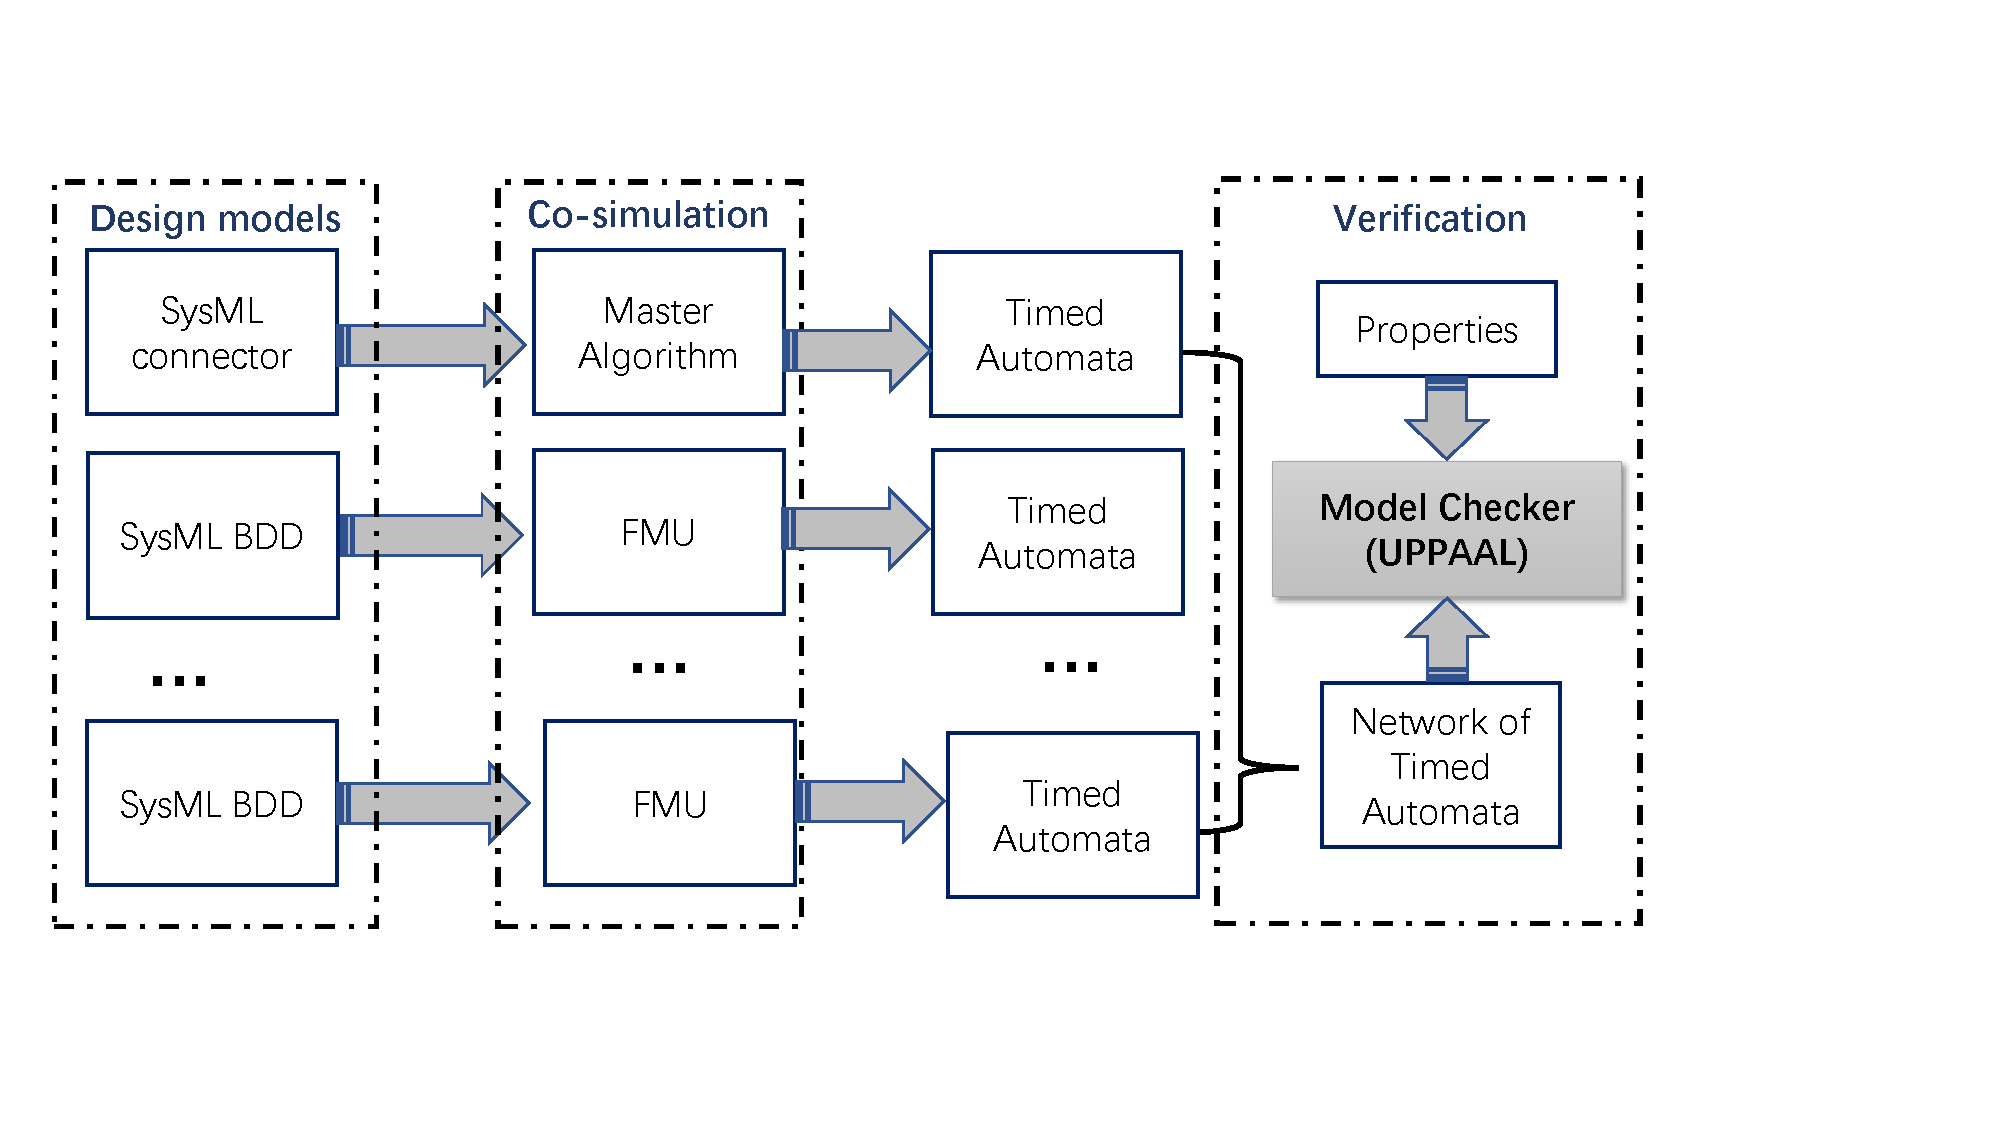
\includegraphics[width=3.5in,height=1.6in]{fig/approach.pdf}}
	\caption{A schematic view of our approach.}
	\label{paper-arc}
\end{figure}

\label{sec:fmi}
\subsection{Encoding FMUs into timed automata}
As we can see, there is a semantic gap between FMU and TA. The former focus on the execution sequence of FMU, which specifies the state change process with time passing. Essentially, the execution trace of TA is semantic equivalence to the execution sequence of FMU. Therefore, we can encode FMU into TA to analyse the behavior of FMU component without exploring its internal structure.

Given an FMU $F=(S,U,Y,D,s_{0},set,get,doStep)$, we encode the FMU into a timed automaton $A = (L,X,l_{0},E,E_{i},E_{o},I)$, the congruent relationship between them is as following:
\begin{itemize}
\item
$L$ is a set of finite states. Note that a location of $A$ is the abstraction of a state in $F$.
\item
The initial location of TA $l_{0}$ which $x:=0 \vert x \in X$ is such that $s$ is set to $s_{0}$ of $F$. 
\item
Each input variable $u \in U$ ranges over $E_{i} \cup \{absent\}$.
\item
Each output variable $y \in Y$ ranges over $E_{o} \cup \{absent\}$.
\item
An input event in $e \in E_{i}$ is such that the function $set$ of $F$ sets the input variable $u$ to a given value. 
\item
An output event in $e \in E_{o}$ indicates that the function $get$ of $F$ gets the output variable $y$. The set of values in the $E_{i}$ can be seen as $Y$ of $F$.  
\item
The communication between the network of TA is the same as the I/O dependencies information in FMU. $(u,y) \in D$ denotes that output $y$ depend on input $u$. The output events also depend on the input events in TA.
\item
For any $e \in E$ of A, there is a transition $s \xrightarrow{e} s^{\prime}$, which may be found after the function $doStep$ is executing. For instance, if there is a transition $l \xrightarrow{e} l^{\prime}$ in $A$, at the same time $doStep(s,h)$ may be called which indicates that $F$ accepts the time step $h$ and reaches the new state $s^{\prime}$. However, $F$ maybe rejects the time step, if there is a rollback behavior happens, the transition in TA could be a edge $l^{\prime} \xrightarrow{e} l$, which denotes that a location travels to the former location.

\end{itemize}
\begin{figure}[htbp]
	\centering	{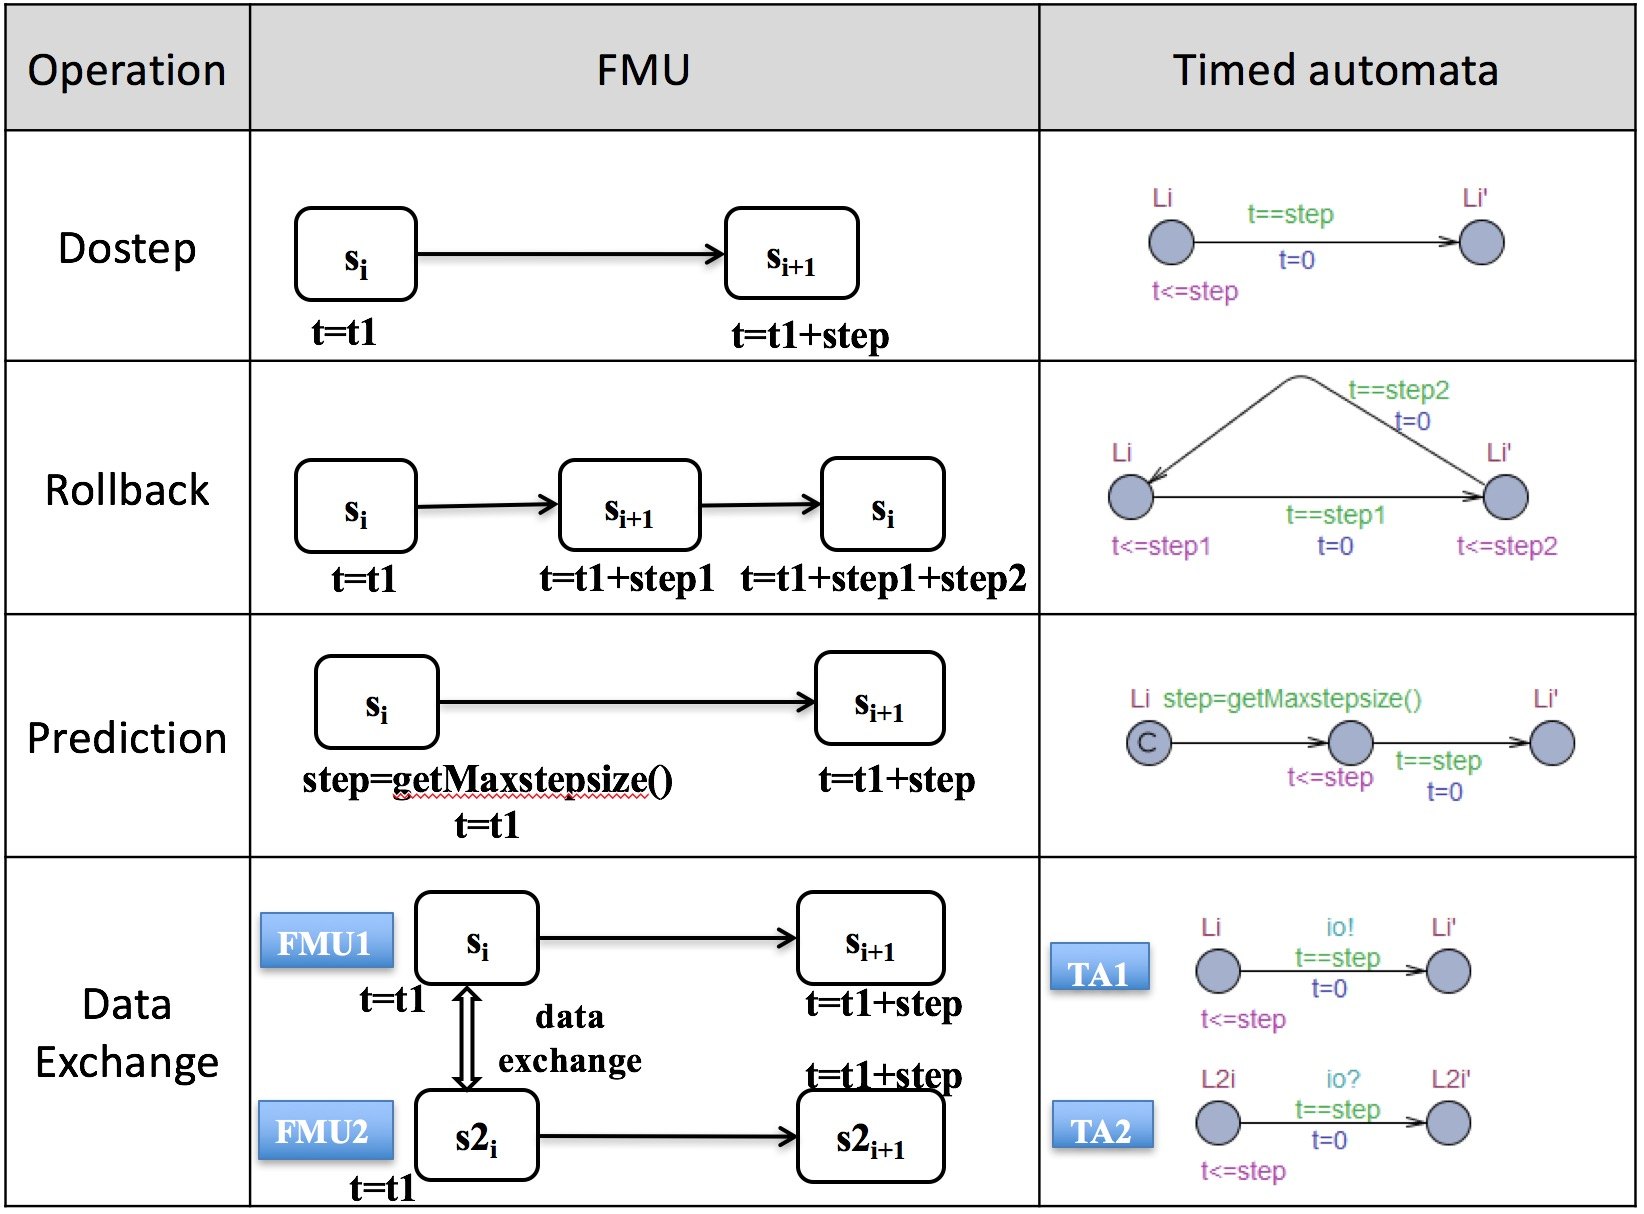
\includegraphics[width=3.5in,height=2.5in]{fig/abstractRole.png}}
	\caption{Encoding rules from FMU to TA.}
	\label{fmutota}
\end{figure}

It is not easy to translate FMU to TA directly, we propose some encoding rules from FMU to TA. As we can see in the Fig.\ref{fmutota}, given a state $s_{i}$ at $t_{1}$ in FMU, the operation $Dostep$ makes FMU reach a new state $s_{i+1}$ at $t_{1}+step$. This situation can be encoded into a transition in TA, in which a location $L_{i}$ delays $step$ time and goes to a new location $L_{i}^{\prime}$.

For the operation $Rollback$, given a state $s{i}$ at $t_{1}$ in FMU, the FMU will do a step1 to $s_{i+1}$ at $t_{1}+step1$, and then, the operation $rollback$ makes FMU reach the former state $s_{i}$. For this situation, it can be encoded as: location $L_{i}$ delays step1 time and reach a new location $L_{i}^{\prime}$ after a transition, next returns to the former Location $L_{i}$. 

For the operation $prediction$, given a state $s_{i}$, FMU can get max step size ($step$) for next step, and then reach a new state $s_{i+1}$ at $t_{1}+step$. For TA, it gets max step size in location $L_{i}$, then it delays $step$ time and reach a new location $L_{i}^{\prime}$ .

For data exchange between two FMUs in state $s_{i}$ at $t_{1}$, they exchange data at $t_{1}$ and then do the same step to $s_{i+1}$. In TA, there will be a signal $io$ to make the two FMUs do the same step from $L_{i}$ to $L_{i+1}$ after data exchange.

Although there are semantic gaps between FMUs and timed automata, we provide appropriate encoding rules to formalism FMU with timed automata. It lays the foundation for analyse FMI co-simulation with timed automata-based model checking.